\documentclass[12pt]{article}


%\setlength{\textheight}{8.8 in}
%\setlength{\textwidth}{6.8 in}
%\setlength{\hoffset}{-.15in}
%\setlength{\voffset}{-0.4 in}
%\setlength{\oddsidemargin}{0pt}
%\setlength{\evensidemargin}{0pt}

%\setlength{\oddsidemargin}{0pt}
%\setlength{\evensidemargin}{0pt}

%\special{papersize=8.5in,11in}
%\setlength{\pdfpageheight}{\paperheight}
%\setlength{\pdfpagewidth}{\paperwidth}
%\newcommand{\K}{ {\rm K}}
%\newcommand{\bigO}{{O\tilde{\phantom{\imath}}}}
%\newcommand{\tbigO}{\widetilde{\mathcal{O}}}

\usepackage{setspace}
\singlespacing
\usepackage{url}
\usepackage{graphicx}
\usepackage{times}
\usepackage{color}
\usepackage{hyperref}
\usepackage{amsfonts}
\usepackage[margin=0.75in]{geometry}
%\setcounter{page}{1}
%\pagestyle{myheadings}
\makeatletter
%\renewcommand{\@oddhead}{Kimon Fountoulakis \hfill}%
\renewcommand{\@evenhead}{\@oddhead}%

\begin{document}

\begin{center}
{Open Postdoc position, starting data January 1, 2021, salary 90,000 CAD/year: \\\vspace{0.2cm} \bf Parallel and Communication Efficient Algorithms For Large-Scale Graph-Based Machine Learning} \\\vspace{0.2cm} {OpAL Lab, David R. Cheriton School of Computer Science, University of Waterloo}\\
\end{center}

We are looking for a postdoctoral research associate for our research group at the University of Waterloo.\ Our goal is to develop parallel and communication efficient algorithms for large-scale graph-based machine learning.\ 
Example algorithms and applications include but not limited to: optimization algorithms for local graph clustering and optimization algorithms for training graph neural networks for node classification, link-prediction, community detection, graph classification and graph generation.\
The successful candidate will also collaborate with the \href{https://www.huawei.com/ca/news/ca-en/20161111huawei-and-university-of-waterloo-partner-for-world-class-research-and-innovation}{Waterloo-Huawei Joint Innovation Lab}  and \href{https://cs.uwaterloo.ca/~ssalihog/}{Assistant Professor Semih Salihoglu} with the end goal to develop a new system or support existing systems on graph-based machine learning.\ The candidate will also be part of the \href{https://scicom.uwaterloo.ca}{Scientific Computation Group} and the \href{https://uwaterloo.ca/artificial-intelligence-institute/}{Waterloo Artificial Intelligence Institute}.\\\vspace{-0.3cm}

\noindent \textbf{Preferred education:} PhD in one of the following or other relevant subjects: numerical optimization, scientific computing, parallel computing.\\\vspace{-0.3cm}

\noindent \textbf{Preferred experience:} Experience in implementation of numerical methods in shared/distributed memory computers and GPUs. \\\vspace{-0.3cm}

%Graph neural networks (GNNs) have attracted a lot of attention recently due to their ability to combine node and edge attributes as well as relational information among nodes.
%In fact, GNNs are the most successful and principled models that exist for many prediction tasks on graphs such as node classification, link-prediction, community detection, graph classification
%and graph generation. Most of the effort in the research community is currently put in developing new models, but little effort is put in making GNNs that are scalable or in parallelizing existing GNNs for large-scale data that do not fit the memory of a single machine.
%We propose to develop parallel and communication avoiding optimization algorithms and a distributed system for training large-scale message passing GNNs (MP-GNNs) that use a mixture of CPUs and GPUs.

%The successful candidate will be involved in developing new projects, measurement, data analysis, instrumental design, and supervision of students. He/she will have her/his own project (starting with the investigation of the melting Mott phase), but will be part of a team and help on other projects as well. \\\hspace{0.5cm}

\noindent \textbf{Additional information}
\begin{itemize}
	\item[-] Location: We are located at the University of Waterloo, a vibrant technological hub with \href{https://concept.uwaterloo.ca}{Concept}, \href{https://velocityincubator.com}{Velocity} and \href{https://careers.google.com/locations/waterloo/}{Google} around the block.\ More information about Waterloo \href{https://www.waterloo.ca/en/index.aspx#}{here}, although it's best if information about the region are communicated face-to-face by talking to members of our group or other residents of Waterloo.\vspace{-0.3cm}
	\item[-] Timeline: We start reviewing applications immediately and until the position is filled (we'll mention this on \url{opallab.ml}). The position is initially one year, and will be extended if both parties are satisfied.\vspace{-0.3cm}
	\item[-] Application: If you are interested in working with us as a postdoc, please send me an \href{mailto:kimon.fountoulakis@uwaterloo.ca}{email}. State briefly why you are interested and attach a CV. Important: please insert ``Application Postdoc'' in the subject line. If you are applying to a specific advertisement, note this in your email.
\end{itemize}


\begin{figure}[htb]
  \center
  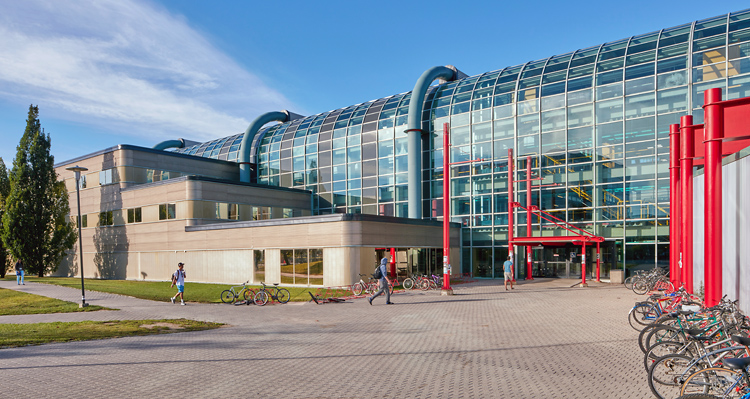
\includegraphics[scale=2.0]{davis-centre-750.jpg}
\end{figure}

\end{document}

